\documentclass[../main.tex]{subfiles}

\begin{document}
\section{Lecture 6 -- SVM}


\begin{remark}
    \begin{center}
        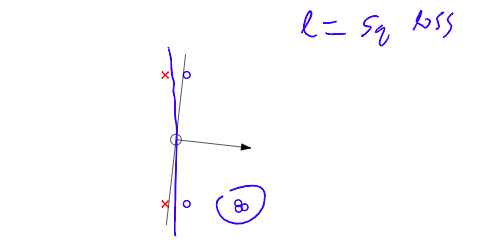
\includegraphics[width=\textwidth,height=\textheight,keepaspectratio]{lecture6_sqloss_tilt}
    \end{center}

    Because square loss seeks to minimize
    distance between the hyperplane determined by a weight vector
    and the location of the point, regardless if the point lies on the correct on the correct side of the hyperplane, the tilt above takes place. We see that, whereas the separating hyperplane was formerly straight and erect, the hyperplane's lower edge now tilts towards the circular cluster to minimize the loss contribution of the cluster's members.
\end{remark}

\begin{remark}
    \begin{center}
        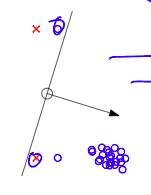
\includegraphics[width=0.5\textwidth,height=0.5\textheight,keepaspectratio]{lecture6_sqloss_bigTilt}
    \end{center}

    If we make a much larger cluster, then the tilting we observed in the previous diagram
    can become extreme. As above, intuition suggests that we devise a means for the separating
    hyperplane to deliberately mispredict on a few samples so that it can predict well
    on the majority of samples.

    \begin{center}
        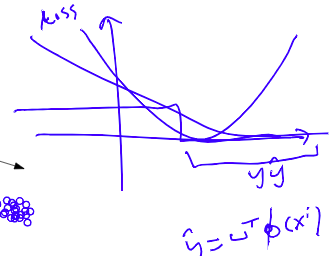
\includegraphics[width=\textwidth,height=\textheight,keepaspectratio]{lecture6_lossFunc}
    \end{center}

    In the diagram above, $\hat{y} = w^T\phi(x^{i})$ and the $x$-axis covers a range of
    values for $y\hat{y}$, and the $y-$axis represents loss. We observe that while
    logistic regression does eventually work well (meaning that its loss does go down
    as we become ``more'' and ``more'' correct, it still incurs error. For ideally,
    the loss function should come closs to following the zero one loss given by
    $1_{\hat{y}y < 1}.$ By this, we mean to suggest that even logistic regression can
    be fed a dataset that causes it to make huge blunders as a consequence (this is not
    verified but intuited by Aahan) of feeding a dataset whose $y\hat{y}$ values are necessarily within a ``small'' neighborhood of $1$. How such a dataset would be constructed is not
    known.

    Recall that the expression below is one term in the loss function for logistic
    regression, and we observe that as $y\hat{y}$ becomes larger and positive, the loss
    incurred drops; it should be noted that we still incur loss, however, even if $y\hat{y} = 1$.
    \[
        \log(1 + \exp{(-y^{i} w^T\phi(x^{i}))})
    \]
\end{remark}

\begin{remark}
    To classify the data, we devise a \textit{linear feasibility problem}, which is 

    \[
        \text{Find } w \in \R^2 \st y^{i}w^Tx^{i} > 0 \forall i \in \{1 \dots n\}.
    \]

    Here we assume that, as before, we are classifying points on the euclidean plane.
    Tautologically, this problem is solveable if and only if it is feasible.
\end{remark}

\begin{definition}
    The maximum margin principle chooses $w$ (and thus chooses a hyperplane) such that
    the distance of a hyperplane to its closest surrounding point is minimal. Formally,
    the principle seeks to elicit $w$ to solve

    \[
        \max_{w \in \R^n} \min_{i \in [n]} \frac{y^{i}w^Tx^{i}}{\norm{w_{i}}_2}
    \]

    Here, we restrict our consideration to those $w$ that separate the data. Ie those
    $w$ such that $y^{i}w^T x^{i}> 0 \forall i$.

\end{definition}

\begin{remark}
    Recall the following: Suppose that we wish to find the distance from $x$ to the plane
    determined by $w$. Recall that $w$ also determines the normal vector \footnote{I
    treat the potential problem that $w$ may be augmented by a bias term later.}. Thus,
    finding the distance from $x$ to the plane determined by $w$ is tantamount to running
    an instance of the normal vector $w$ through the point $x$ and then calculating the
    projection of $x$ onto $w$. This is $\norm{x \cos \theta}$ where $\theta$ is the angle
    formed between $x$ and the instance of $w$ running through $x$. This is also equivalent
    to $\norm{\frac{x \cdot w}{\norm{w}}\frac{x}{\norm{x}}}$ by the dot product fomrmula,
    which reduces to $\frac{x \cdot w}{\norm{w}}$. This is what informs the minimum above.
\end{remark}

\begin{proposition}
    \[
        \max_{w \in \R^d} \min_{i \in [n]} \frac{y^{i}w^Tx^{i}}{\norm{w_{i}}_2} = \max_{w \in \R^d} \frac{1}{\norm{w}} \st ` \leq y^{i}w^Tx^{i} \forall i \in \{1 \dots n\}
    \]
\end{proposition}

\begin{proof}
    \begin{align*}
        \max_{w \in \R^d} \min_{i \in [n]} \frac{y^{i}w^Tx^{i}}{\norm{w}_2} \\
        = \max_{w \in \R^d, r \geq 0}  \frac{r}{\norm{w}_2} \st r \leq y^{i}w^Tx^{i}  \qquad \forall i \\
        = \max_{w \in \R^d, r \geq 0}  \frac{r/r}{\frac{\norm{w}_2}{r}} \st r \leq y^{i}w^Tx^{i}  \qquad \forall i \\
        = \max_{w \in \R^d, r \geq 0}  \frac{1}{\norm{w/r}_2} \st r \leq y^{i}w^Tx^{i}  \qquad \forall i \\
        = \max_{w \in \R^d, r \geq 0}  \frac{1}{\norm{w/r}_2} \st 1 \leq y^{i}(w/r)^Tx^{i}  \qquad \forall i \\
        = \max_{w \in \R^d}  \frac{1}{\norm{w}_2} \st 1 \leq y^{i}(w)^Tx^{i}  \qquad \forall i \\
        = \min_{w \in \R^d}  \frac{1}{2}\norm{w}^2 \st 1 \leq y^{i}(w)^Tx^{i}  \qquad \forall i \\
        \intertext{Note that the previous problem is convex} \\
    \end{align*}
\end{proof}


\begin{theorem}
    The dual for the separable case is

    \[
        D(\alpha) \coloneq \inf_{w \in \R^d} L(w, \alpha) = \begin{cases}
            \sum_{i=1}^{n}\alpha_i - \frac{1}{2}\norm{\sum_{i=1}^{n}\alpha_iy^{i}x^{i}}^2 & \alpha \geq 0 \\
            -\infty \\
        \end{cases}
    \]
\end{theorem}

\begin{proof}
    \begin{align*}
                = \min_{w \in \R^d}  \frac{1}{2}\norm{w}^2 \st 1 \leq y^{i}(w)^Tx^{i}  \qquad \forall i \\
                \intertext{Compells a Lagrangian, which is:} \\
                = \frac{1}{2}\norm{w}^2 + \sum_{i=1}^{n}\alpha_i(1 - y^{i}w^Tx^{i}) \numberthis{1} \\
                \intertext{Where $\alpha_{i} \geq 0.$} \\
                \intertext{Now differentiate this and set it to $0$} \\
                0 = w^T - \sum_{i=1}^{n}\alpha_{i}y^{i}\left( x^{i} \right)^T \\
                w = \sum_{i=1}^{n}\alpha_{i}y^{i}\left( x^{i} \right) \\
                \intertext{Now substitute this into \ref{1}}
                = \frac{1}{2}\norm{\sum_{i=1}^{n}\alpha_{i}y^{i}\left( x^{i} \right)}^2 + \sum_{i=1}^{n}\alpha_i(1 - y^{i}(\sum_{i=1}^{n}\alpha_{i}y^{i}\left( x^{i} \right))^Tx^{i}) \\
                = \frac{1}{2}\norm{\sum_{i=1}^{n}\alpha_{i}y^{i}\left( x^{i} \right)}^2 + \sum_{i=1}^{n}\alpha_i - \sum_{i=1}^{n}y^{i}(\sum_{i=1}^{n}\alpha_{i}y^{i}\left( x^{i} \right))^Tx^{i} \\
                \intertext{Notice that the right most expression is really $-\norm{w}^2$.}\\
                = \sum_{i=1}^{n}\alpha_i - \frac{1}{2}\norm{\sum_{i=1}^{n}\alpha_iy^{i}x^{i}}^2  \\
    \end{align*}
\end{proof}

\begin{remark}
    The foregoing all assumed that we were working in the separable case. If we cannot satisfy the feasibility condition:

    \[
        y^{i}w^Tx^{i} > 0 \qquad \forall i 
    \]

    we introduce a set of slack variables $\{\xi | \xi \geq 0 \}$ and reframe the feasibility problem as an optimization problem

    \[
        \min_{\{\xi\}} \sum_{i=1}^{n}\xi_{i} \qquad \st y^{i}w^Tx^{i}  > 0 - \xi_{i} \qquad \forall i
    \]

    The idea is that $\{\xi_{i}\}$ represent the minimal amount of translations necessary
    for a feasible problem to be obtained.
\end{remark}

\begin{remark}
    Note that the previous reformulation is a slackening of the feasibility problem. To slacken the actual optimizaiton problem, we define the Soft Margin SVM, as follows:
\end{remark}

\begin{definition}
    The Soft Margin SVM (for the non-separable case) solves the following problem:

    \[
        \min_{w \in \R^d, \xi \in \R^n} \frac{1}{2}\norm{w}^2 + C\sum_{i=1}^{n}\xi_{i} \quad \st 1 - \xi \leq y^{i}w^Tx^{i} \qquad \forall i \in \{1 \dots n\}
    \]

    This is obtained by slackening the former separable optimization problem

    \begin{align*}
        \min_{w \in \R^d}  \frac{1}{2}\norm{w}^2 \st 1 \leq y^{i}(w)^Tx^{i}  \qquad \forall i \\
        \intertext{Now add $\sum_{i=1}^{n}\xi_{i}$ to the LHS and subtract $\xi_{i}$ from the RHS.} \\
        \min_{w \in \R^d, \xi \in \R^n} \frac{1}{2}\norm{w}^2 + C\sum_{i=1}^{n}\xi_{i} \quad \st 1 - \xi \leq y^{i}w^Tx^{i} \qquad \forall i \in \{1 \dots n\} \\
        \intertext{Where $C > 0$ is effectively a regularizer} \\
    \end{align*}

\end{definition}

\begin{remark}
    To develop intuition for what $C$ does, let us divide $C$ from
    \[
        \min_{w \in \R^d, \xi \in \R^n} \frac{1}{2}\norm{w}^2 + C\sum_{i=1}^{n}\xi_{i} \quad \st 1 - \xi \leq y^{i}w^Tx^{i} \qquad \forall i \in \{1 \dots n\} \tag{$\gamma$}\\
    \]

    to obtain

    \[
        \min_{w \in \R^d, \xi \in \R^n} (1/C)\frac{1}{2}\norm{w}^2 + \sum_{i=1}^{n}\xi_{i} \quad \st 1 - \xi \leq y^{i}w^Tx^{i} \qquad \forall i \in \{1 \dots n\} \\
    \]
    
    Let $(1/C) = \lambda$.

    \[
        \min_{w \in \R^d, \xi \in \R^n} \lambda\frac{1}{2}\norm{w}^2 + \sum_{i=1}^{n}\xi_{i} \quad \st 1 - \xi \leq y^{i}w^Tx^{i} \qquad \forall i \in \{1 \dots n\} \\
    \]

    Now we make the following observations:

    \begin{outline}
        \1 As $\lambda \to \infty$, $w$ becomes more constrained so that more freedom is
        given to $\{\chi_{i}\}.$ Hence, in the original formulation in $(\gamma)$, we see that
        the smaller $C$ is the more flexibility we give to $\{\chi_{i}\}$. What does it mean
        to be more flexible? Similarly, as $\lambda \to 0$, $w$ becomes more and more flexible and
        we care more about minimizing the loss incurred by the $\{\chi_{i}\}$ so $\{\chi_{i}\}$ become less flexible.
    \end{outline}

    \begin{unresolved}
        What is this tradeoff? Can we motivate it more rigorously?
    \end{unresolved}
\end{remark}

\begin{theorem}
    \[
        \min_{w \in \R^d, \xi \in \R^n} \lambda\frac{1}{2}\norm{w}^2 + \sum_{i=1}^{n}\xi_{i} \quad \st 1 - \xi \leq y^{i}w^Tx^{i} \qquad \forall i \in \{1 \dots n\} \\
    \]

    is equivalent to

    \[
        \min_{w \in \R^d} \lambda\frac{1}{2}\norm{w}^2 + \sum_{i=1}^{n}\text{\textit{l}-hinge}(y^{i}w^Tx^{i}) \qquad \forall i \in \{1 \dots n\} \\
    \]

    where \textit{l}-hinge applied to $x$ is $\max\{1 - x, 0\}$.

\end{theorem}

\begin{proof}

    \begin{align*}
        \min_{w \in \R^d, \xi \in \R^n} \lambda\frac{1}{2}\norm{w}^2 + \sum_{i=1}^{n}\xi_{i} \quad \st 1 - \xi \leq y^{i}w^Tx^{i} \qquad \forall i \in \{1 \dots n\} \\
        = \min_{w \in \R^d} \min_{\xi \in \R^n} \lambda\frac{1}{2}\norm{w}^2 + \sum_{i=1}^{n}\xi_{i} \quad \st 1 - \xi \leq y^{i}w^Tx^{i} \qquad \forall i \in \{1 \dots n\} \\
        \intertext{Notice that once $w$ is determined, there is an obvious choice, however,
        for the argument $\xi$ such that the resultant value is minimized.} \\
        \intertext{We obtained this by manipulating the constraint inequality} \\
        = \min_{w \in \R^d} \lambda\frac{1}{2}\norm{w}^2 + \sum_{i=1}^{n}(1 - y^{i}w^Tx^{i})  \\
        \intertext{Recall, however, that even if take $\xi_{i}$ to be $1 - y^{i}w^Tx^{i}$ in order to maximally slacken the inequality $1  - y^{i}w^Tx^{i} \leq \xi_{i}$, we must have $\xi_{i} \geq 0$, whence we replace $1 - y^{i}w^Tx^{i}$ with} \\
        = \min_{w \in \R^d} \lambda\frac{1}{2}\norm{w}^2 + \sum_{i=1}^{n}(\max\{0,1 - y^{i}w^Tx^{i}\})  \\
    \end{align*}
    
\end{proof}

\begin{remark}
    \begin{center}
        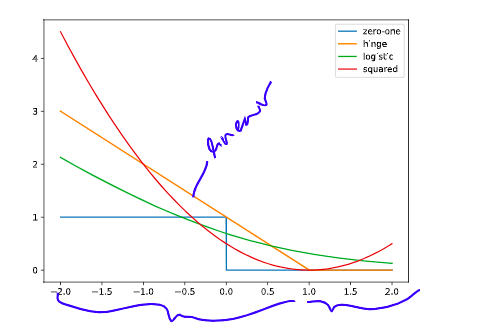
\includegraphics[width=\textwidth,height=\textheight,keepaspectratio]{lecture6_lossGraphs}
    \end{center}

    The graph above plots $y\hat{y} = y^{i}w^Tx^{i}$ on the $x-$axis and the different loss functions on the $y$-axis: $(1 - y\hat{y})^2$, $1_{y\hat{y} \leq 1}$, $\sigma(y\hat{y})$ and then $\mathcal{L}(\hat{y}y)$. Hinge loss does not penalize correctness, and it penalizes misclassification linearly; that is $e(y_{1}\hat{y_{1}}) = 2e(y_{2}\hat{y_{2}}) \iff y_{1}\hat{y_{1}} = 2(y_{2}\hat{y_{2}}),$ where $e$ signifies error.
\end{remark}

\begin{remark}
    \begin{center}
        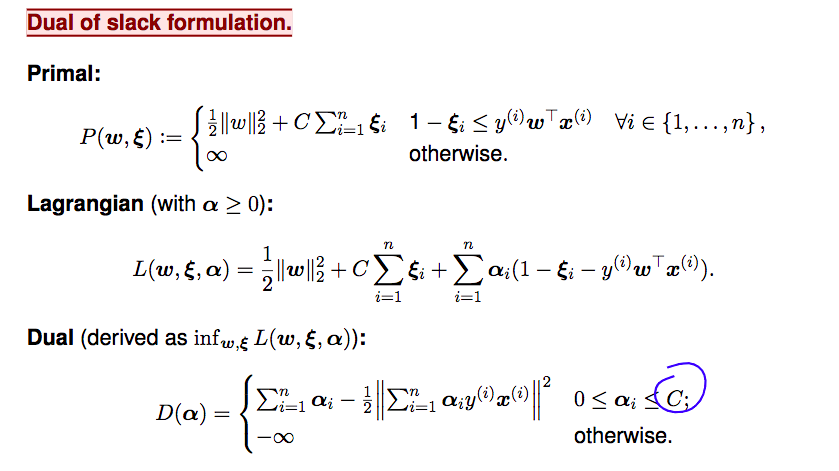
\includegraphics[width=\textwidth,height=\textheight,keepaspectratio]{lecture6_dualSlack}
    \end{center}

    If we try to solve the primal problem for the slack formulation, then when we optimize
    the Lagrangian by minimizing over $w, \xi$, we take the gradient with respect to $w$
    and then obtain $w = \sum_{i=1}^{n}\alpha_{i}y^{i}x^{i}$.

    \begin{unresolved}
        It is not known how they conclude that the optimal value for $\{\xi\}$ is somehow
        related to $\sup_{\xi \geq 0} \xi(C - \alpha_i)$.

        \textbf{Solution:}

        We seek to maximize the dual function, which is obtained as the infimum of the
        Langrangian. If we allowed $\alpha > C$, note that we could arbitrarily then
        minimize the dual, for then $\xi(C - \alpha_i) \to -\infty$. To foreclose this
        possibility, we therefore compel that $\alpha \leq C$.
    \end{unresolved}

    It will turn out that $0 \leq \alpha_{i} \leq C$, so that the only values contributing
    to the optimal value of $w$, which was found to be $\sum_{i=1}^{n}\alpha_i y^{i}x^{i}$
    are those $i$ such that $\alpha_i > 0$. This is impactful as follows:

    Suppose that we optimize the dual program 

    \[
        \max_{\alpha \in [0,C]^n} \sum_{i=1}^{n}\alpha_{i} - \frac{1}{2}\norm{\sum_{i=1}^{n}\alpha_{i}y^{i}x^{i}} \tag{$\beta$}
    \]

    and obtain a corresponding optimal value for $\alpha$. Now let us solve this problem again and, this time, discard those $(x^{i}, y^{i})$ such that $\alpha^{i} = 0$. Now try once more to solve $(\beta)$ -- and we will obtain a vector $\alpha_2$ such that the $\alpha$ when restricted to its coordinates greater than $0$ is precisely $\alpha_2$. We call the $x_i$ whose $\alpha^i > 0$ the support vectors.
\end{remark}

\begin{remark}
    Notice that we can rewrite $(\beta)$ above to be

    \[
        \max_{\alpha \in [0,C]^n} \sum_{i=1}^{n}\alpha_{i} - \frac{1}{2}\sum_{i,j=1}^{n}\alpha_{i}\alpha_{j}y^{i}y^{j} (\phi(x_{i})^T \phi(x_{j}))
    \]

    When we define $k(x^{i}, x^{j})$ to be $(\phi(x_{i})^T \phi(x_{j}))$, we call the resultant $k$ a kernel.
\end{remark}

\begin{proposition}
    If $\phi(x)$ is the feature transform function for a problem, then after finding the 
    optimal $\{\alpha_{i}\}$ from using an SVM, the prediction function to determine which
    side of a hyperplane a point lies on is

    \[
        f(x) = \sum_{i=1}^{n}\alpha^{i}y^{i}k(x^{i},x)
    \]
\end{proposition}

\begin{proof}
    Recall that the optimal value of $w$, found from the Lagrangian, was found to be

    \[
        w = \sum_{i=1}^{n}\alpha_{i}y^{i}\phi(x^{i})
    \]

    Recall, further, that we decide the label of a point using $sgn(w^Tx)$. Whence,
    substituting $w$ as above, we now have:

    \begin{align*}
        \left(\sum_{i=1}^{n}\alpha_{i}y^{i}\phi(x^{i})\right)^Tx  \\
        = \left(\sum_{i=1}^{n}\alpha_{i}y^{i}k(x^{i}, x)\right)  \\
    \end{align*}
\end{proof}

\begin{proposition}
    Suppose that we want to perform gradient descent on hinge loss using only one training
    example. Then the update rule is

    \[
        w' \coloneq (1 - \lambda)w + yx \cdot 1_{[yw^Tx < 1]}
    \]

    where we let $\alpha = 1$ be the step size.
\end{proposition}

\begin{proof}
    Recall that hinge loss is 

    \[
        \mc{L}_{\text{hing}}(yw^Tx) + \lambda \norm{w}^2/2 = \max\{1 - yw^Tx, 0\} + \lambda \norm{w}^2/2
    \]

    Whenever $yw^Tx < 1$, the loss function is therefore

    \[
        1 - yw^Tx + \lambda \norm{w}^2/2 \text{ and } \lambda \norm{w}^2/2 \text{ otherwise}.
    \]

    Taking the derivative of the first gives us (and transposing so that the gradient is a column vecto)

    \[
        -yx + \lambda w \text{ and the other derivative is } \lambda w
    \]

    Exclusively working with the first derivative, compute

    \[
        w \coloneq w - \alpha(-yx + \lambda w) = w(1 - \lambda) + \alpha yx 1[yw^Tx < 1]
    \]

    where the final term is added, to account for the fact that we looked at a piecewise
    component of hinge loss to obtain the loss function which we subsequently differentiated.

    Let $\alpha = 1$ to obtain the form in the proposition.
\end{proof}

\begin{remark}
    This update rule has a geometric interpretation: If $yw^Tx < 1$, meaning that our
    prediction is off, then update the hyperplane normal vector by tilting it in the direction
    of $yx$. If $0 < \lambda < 1$, then we also keep the value of $(1 - \lambda)w$ small.
\end{remark}

\section{Lecture 7}


\begin{remark}
    \begin{center}
        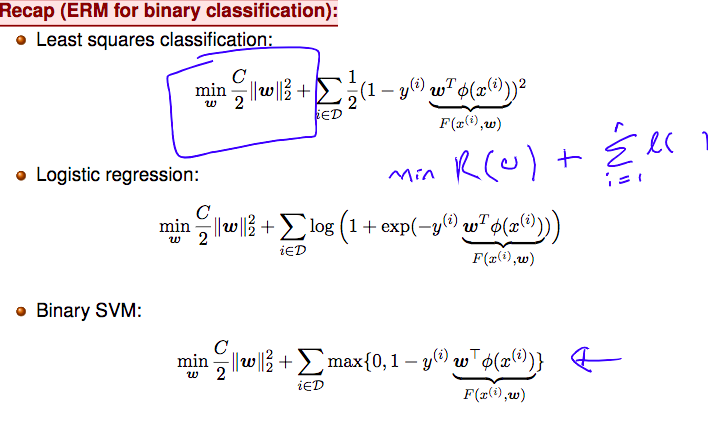
\includegraphics[width=\textwidth,height=\textheight,keepaspectratio]{lecture7_lossFuncs}
    \end{center}

    Note that all loss functions studied to date are of the form Regularization  + ERM.
\end{remark}

\begin{definition}
    When a loss function can be interpolated into another loss function, we mean that there
    exists a function $F(x, \e)$ that can be manipulated to be either $l_1$ or $l_2$, where
    $l_1$ and $l_2$ are the loss functions. This often involves some limiting procedure involving $\e$.
\end{definition}

\begin{theorem}
    We can interpolate log loss into SVM loss.
\end{theorem}

\begin{remark}
    \begin{center}
        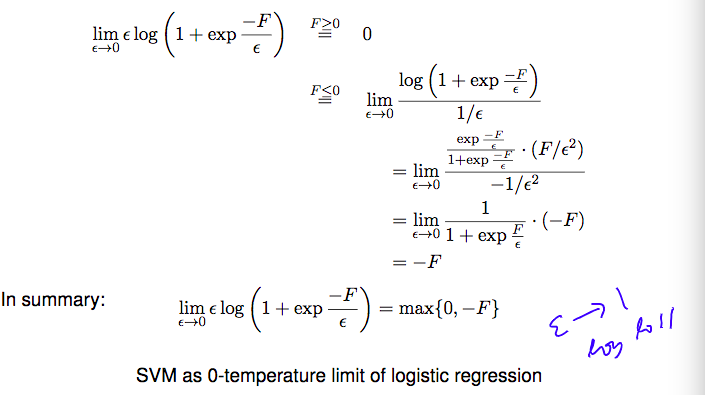
\includegraphics[width=\textwidth,height=\textheight,keepaspectratio]{lecture7_interp}
    \end{center}

    Note that we apply L'Hoptial's rule when our limit expression is of the form $0/0$.
\end{remark}

\begin{remark}
    \begin{center}
        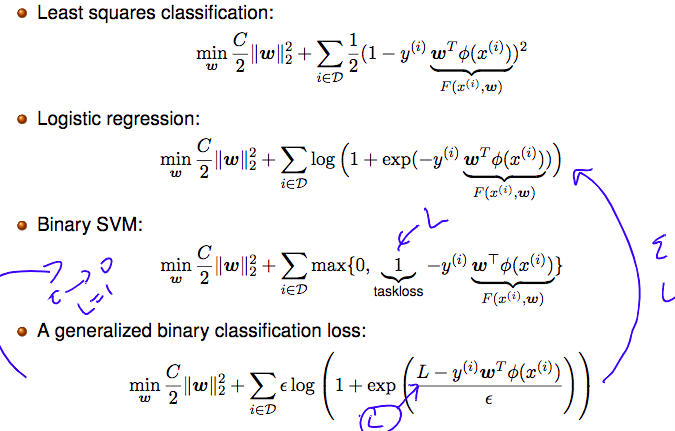
\includegraphics[width=\textwidth,height=\textheight,keepaspectratio]{lecture7_generalLoss}
    \end{center}

    By choosing different values for $L$ and $\e$ in the generalized loss function, we can
    get different loss functions.
\end{remark}

\begin{definition}
    To classify between $K$ classes, a 1 versus all classifier constructs $K-1$ classifiers. Each classifier, say $C^{i}$, labels if an input belongs to class $i$ or else belongs to some other class.
\end{definition}

\begin{remark}
    \begin{outline}
        \1 The $1$ versus rest classifier is problematic insofar as:
        \2 The data used to train a particular classifier, say $C^{i}$, is likely imbalanced:
        \3 If all classes had $m$ samples each, then we would constructing a classifier to correctly categorize $m$ samples as belonging to one class and $m(d-1)$ samples as belonging to another class.
        \2 We may produce more than one good answer or no good answer:
        \3
            \begin{center}
                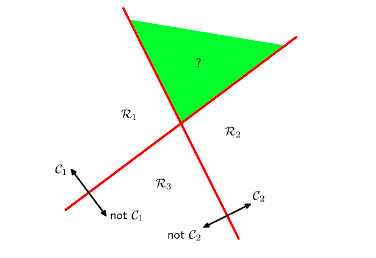
\includegraphics[width=\textwidth,height=\textheight,keepaspectratio]{lecture7_oneVsAll}
            \end{center}
        \4 Here, observe that both $C_1$ and $C_2$ are alleged labels for the shaded region.
        \1 It is good insofar as it requires $O(k)$ classifiers.
    \end{outline}
\end{remark}

\begin{definition}
    To classify $K$ classes, a 1 versus 1 clasifier creates binary classifiers for each
    pair of classes. Once all $k(k-1)/2$ classifiers have been constructed, given a sample
    $x$, we then give a label for $x$ using each of the classifiers. Whichever class
    achieves a plurality over $x$ is set to be the class label of $x$.
\end{definition}

\begin{remark}
    \begin{outline}
        \1 This is problematic insofar as:
        \2 Each classifiers may have very little data to work with
        \2 There are $O(K^2)$ classifiers.
        \2 Two-way preferences may not be transitive:
        \3
            \begin{center}
                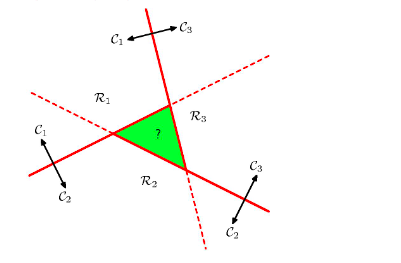
\includegraphics[width=\textwidth,height=\textheight,keepaspectratio]{lecture7_poorTransitivity}
            \end{center}

        \4 Choose a point in the green region. Observe that it would be given the class
        label $C_2$ over $C_1$ and $C_3$ over $C_2$; that does not imply, however, that
        it would be given the label $C_3$ over $C_1$; indeed, $C_1$ is preferred over
        $C_3$ here.
        \1 This is beneficial because:
        \2 The data required to build each classifier is more likely to be balanced than
        the data required to build each 1 versus all classifier.
        \2 We can train the classifiers in parallel.
    \end{outline}
\end{remark}

\begin{definition}
    The multinomial classifier for classification over $K$ classes constructs $K-1$
    weight vectors $w_{1} \dots w_{K-1}$. \footnote{A technicality is that we need the probability function to include a summation over all $K$ weight vectors in its denominator; however, when we train our model, we only need to perform updates for the first $K-1$ weight vectors, and by obtaining probabilities over all the toer} After these vectors are constructed, given
    a sample $x$, we predict its label to be the class $i$ such that

    \[
        \bb{P}(Y = y^{i} | x) = \frac{\exp(w_{i}^T\phi(x))}{\sum_{j=1}^{K}\exp(w_{j}^T\phi(x))}
    \]

    is maximal over all other labels. To train the $\{w_{i}\}$, we do the following:
    set $w = [w_{1} \dots w_{K}]$ and then minimize the loss function:

    \[
        \arg \max_{w} \prod_{(x^{i},y^{i}) \in D} \bb{P}(Y = y^{i} | x^{i}) = \arg \min_{w} 
        -\sum_{(x^{i}, y^{i})} \log(\bb{P}(Y = y^{i} | x^{i})) = \mc{L}
    \]

    Performing Gradient Descent, we then minimize over

    \[
        \begin{bmatrix}
            w_1 \\
            \vdots \\
            w_{K} \\
        \end{bmatrix} - \alpha_{i} \begin{bmatrix}
            \nabla_{w_1} \mc{L} \\
            \vdots \\
            \nabla_{w_{K}} \mc{L} \\
        \end{bmatrix}
    \]
\end{definition}

\begin{example}
    Suppose that we perform this procedure for two classes. One can show, in that case,
    that we end up finding that $w_1 = -w_2$.
\end{example}

\begin{example}
    We provide some intuition on how maximizing the ``margin'' is related to the
    optimization problem:

    \[
        \min_{w} \frac{1}{2}\norm{w}^2 \st y^{i}w^T\phi(x^{i}) \geq 1 \forall (x^{i},y^{i}) \in \mc{D}
    \]

    Suppose that we have data configured as follows:

    \begin{center}
        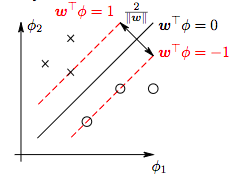
\includegraphics[width=\textwidth,height=\textheight,keepaspectratio]{lecture7_svmIntuition}
    \end{center}

    Suppose that $w^Tu_1 = 1$ (this is labeled as $w^T\phi = 1$ in the diagram) and that $w^Tu_2 = 2$. Then the following computations can be done and we observe that the distance from $u_1$ to $u_2$ is $\frac{2}{\norm{w}}$.
    \begin{center}
        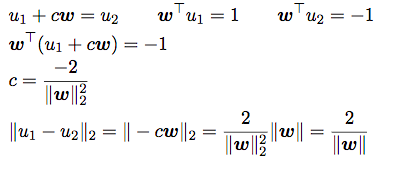
\includegraphics[width=\textwidth,height=\textheight,keepaspectratio]{lecture7_svmIntuitionMath}
    \end{center}

    Minimizing $\frac{2}{\norm{w}}$ is tantamount to minimizing the norm (and hence the square of the norm).
\end{example}

\begin{definition}
    Suppose that we have labels $y \in \{0 \dots K-1\}$ and corresponding class vectors $w_{y}$. We want to so finely choose our class vectors that we have:

    \begin{center}
        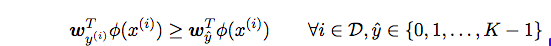
\includegraphics[width=\textwidth,height=\textheight,keepaspectratio]{lecture7_svmMulticlassConstraint}
    \end{center}
\end{definition}

\begin{definition}
    If we make this definition where $\delta(y^{i} = Z)$ is really $1_{y^{i} = Z}$.
    \begin{center}
        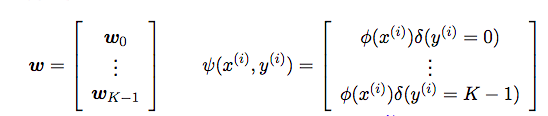
\includegraphics[width=\textwidth,height=\textheight,keepaspectratio]{lecture7_equivalentForm}
    \end{center}

    then observe that

    \[
        w^T\left( \psi(x^{i},y^{i}) - \psi(x^{i},\hat{y}) \right) \geq 1 - \xi^{i} \qquad \forall i,\hat{y}
    \]
    
    is equivalent to

    \[
        w_{y^{i}}^T\phi(x^{i}) - w_{\hat{y}}^T\phi(x^{i}) \geq 1 - \xi^{i} \qquad \forall i, \hat{y}
    \]

    which informs \\

    \begin{center}
        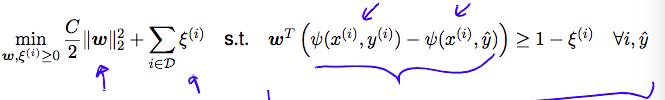
\includegraphics[width=\textwidth,height=\textheight,keepaspectratio]{lecture7_equivalentFormOpt}
    \end{center}

    Using the same technique that we used earlier to define hinge loss, observe that
    we now need to minimize $\xi^{i}$ while ensuring that
    \[
        \xi^{i} \geq 1 - w^T\left( \psi(x^{i},y^{i}) - \psi(x^{i},\hat{y}) \right) \forall i, \hat{y}
    \]

    If we fix a particular $i$, so that we want to determine the minimum value of $\xi^{i}$,
    then we declare $\xi^{i}$ to be at least

    \[
        \max_{\hat{y}} (1 - w^T\left( \psi(x^{i},y^{i}) - \psi(x^{i},\hat{y}) \right) \forall i, \hat{y})
    \]

    and $0$ if this value is negative. Whence we obtain the objective function

    \[
        \min_{w} \frac{C}{2}\norm{w}^2 + \sum_{i \in D}^{}\max\{0 , \max_{\hat{y}} (1 - w^T\left( \psi(x^{i},y^{i}) - \psi(x^{i},\hat{y})) \right)\}
    \]

    Notice that $1 - w^T\left( \psi(x^{i},y^{i}) - \psi(x^{i},\hat{y}\right)$ is precisely $1$
    when $\hat{y} = y^{i}$ so that the expression $\max_{\hat{y}} 1 - w^T\left( \psi(x^{i},y^{i}) - \psi(x^{i},\hat{y})\right) \geq 0$.

    \[
        \max_{\hat{y}} 1 - w^T \left( \psi(x^{i},y^{i}) - \psi(x^{i},\hat{y}) \right)
    \]

    Since the outer maximum will unambigously choose the second parameter, the objective becomes
    \[
        \min_{w} \frac{C}{2}\norm{w}^2 + \sum_{i \in D}^{} \max_{\hat{y}} (1 - w^T\left( \psi(x^{i},y^{i}) - \psi(x^{i},\hat{y})) \right)
    \]

    Only the first term after the summation depends on $\hat{y}$, so we have

    \[
        \min_{w} \frac{C}{2}\norm{w}^2 + \sum_{i \in D}^{} \max_{\hat{y}} \left(1 + w^T\left( \psi(x^{i}, \hat{y})\right)\right) - w^T\left( \psi(x^{i},y^{i})\right) 
    \]

    \breathe

    This is the Multiclass SVM objective function.
    
\end{definition}

\begin{remark}
    We can also perform interpolation of the SVM to obtain the multiclass logistic regression equation and vice versa.

    \begin{center}
        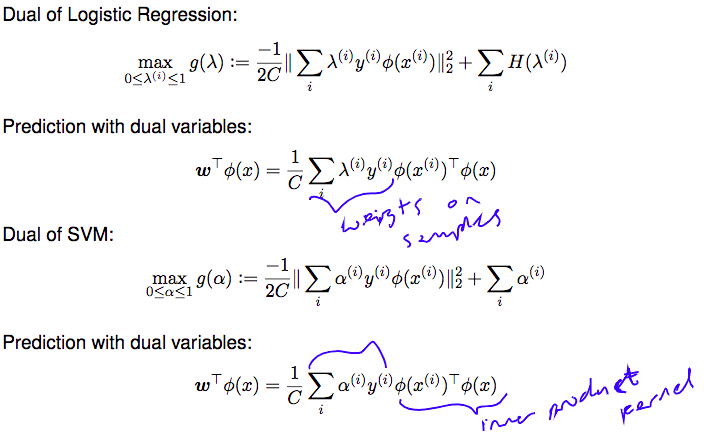
\includegraphics[width=\textwidth,height=\textheight,keepaspectratio]{lecture7_logisticSVM}
    \end{center}

    Notice that both the SVM predictiona and logistic regression (after training) have are similar in form; note especially the inner product $\left(\phi(x^{i})\right)^T\phi(x)$. We can replace the expression $\left(\phi(x^{i})\right)^T\phi(x)$ by $k(x^{i},x)$ where $k$ is some function in which the action of $\phi$ is implicit. This is practically significant: in a training algorithm, instead of constructing $phi(x)$ and then performing the dot product, just replace the call to $\phi(x)^T\phi(x)$ with one to $k(x^T,x)$. There are many kernels we can choose from, however! Can we choose any function? -- no! We can choose only those kernels that can be induced as the inner product of two feature vectors obtained via some feature transformation.

    There happen to be two tests for this, the theory behind which is presently UNRESOLVED. The first is to form the Gram matrix where $K_{i,j} = k(x^{i}, x^{j})$ and, supposedly, $K$ is positive definite if and only if $k$ is a valid kernel. The second is to decompose the kernel into and from known kernels.


    These are valid means of constructing new kernels (UNRESOLVED):
    \begin{center}
        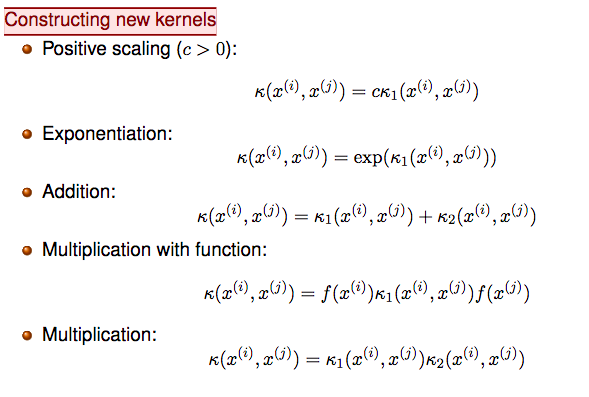
\includegraphics[width=\textwidth,height=\textheight,keepaspectratio]{lecture7_validKernelOps}
    \end{center}
\end{remark}

\section{Lecture 8 -- Deep Learning I}

\section{Lecture 9 -- Deep Learning II}

\section{Lecture 10 -- Trees, Bagging and Boosting}


    \begin{definition}
        A decision tree is a classifier that walks an input down a tree. At each node of the
        tree, a function is applied to the input: if the output is ``positive'' in one sense,
        we go to the right and to the left otherwise.
    \end{definition}

    \begin{center}
        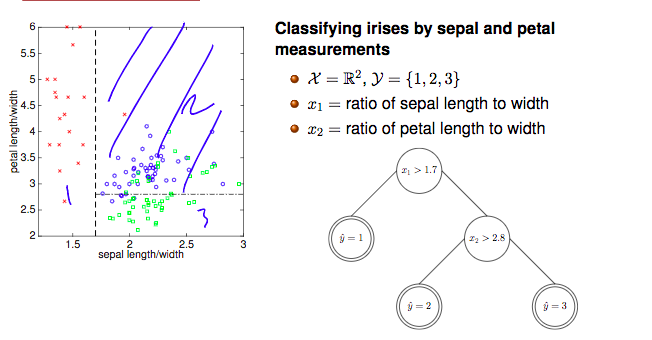
\includegraphics[width=\textwidth,height=\textheight,keepaspectratio]{lecture8_decision_tree}
    \end{center}

    \begin{example}
        In the example above, we see that an input initially goes right if its value is
        greater than $1.7$, and it goes left otherwise. Eventually, when we reach a leaf,
        we have reached the label that we assign to the input. As a consequence of this binary
        decision nature, decision boundaries often end up like looking like the boundary
        structure shown to the left.
    \end{example}

    \begin{center}
        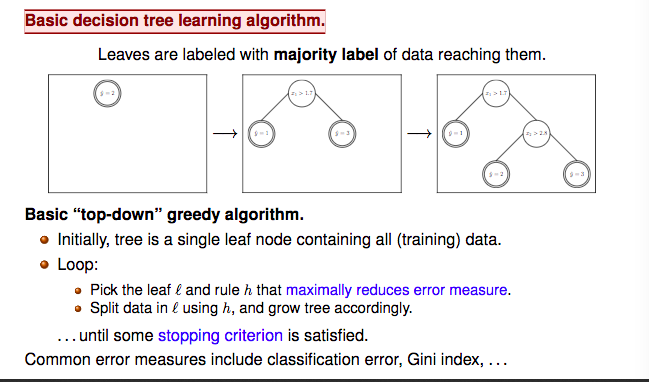
\includegraphics[width=\textwidth,height=\textheight,keepaspectratio]{lecture8_decision_tree_algo}
    \end{center}

    \begin{remark}
       There are two other stopping criterions that are popularly used. The first is to
       stop when the tree reaches a pre-specified size (it is, for some reason, remarked
       in the lecture slide that this involves the choice of some tuning hyperparameters).
       The second is to stop when every leaf is pure (recall that if we begin with a leaf,
       then the leaf is labeled by all labels). This can result in overfitting, however,
       in that we also capture noise, as shown below:
    \end{remark}

    \begin{center}
        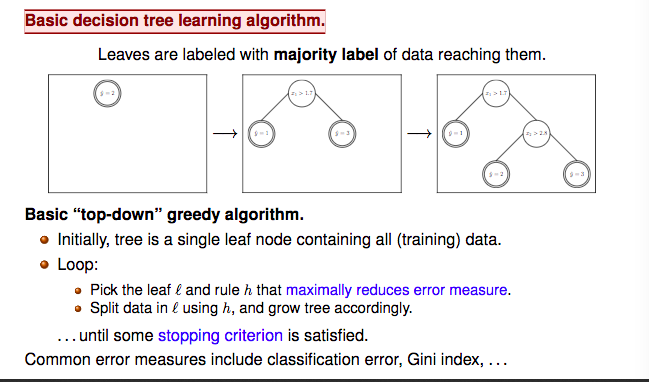
\includegraphics[width=\textwidth,height=\textheight,keepaspectratio]{lecture8_decision_tree_algo}
    \end{center}

    \begin{remark}
        We say that a tree overfits if training error goes to zero as we increase the
        number of tree nodes but the true error, while initially decreasing, eventually
        increases. To underfit, by contrast, is to have both poor training error and poor
        true error. For this reason, there is some regularization done on trees; one
        idea is to remove tree leaves, a strategy called pruning.
    \end{remark}

    \begin{unresolved}
        It is NP hard to determine the smallest decision tree consistent with data.
        I don't know what this means.
    \end{unresolved}

    \begin{definition}
        An ensemble classifier builds multiple classifiers and then classifies an
        example using the majority label of the classifiers that it uses.
    \end{definition}

    \begin{remark}
        If we assume that each classifier is independent and misclassifies with probability
        less than $0.5$ (in the example that follows, the probability of failure is $0.4$),
        then the probability that all classifications are wrong is very small. This follows
        a binomial distribution: $B(n,0.4)$, the results of which are shown below. Note that
        the $x$ axis is a bit nonsensical -- they should really be values of $n$ from $1$
        to $7$.
    \end{remark}

    \begin{center}
        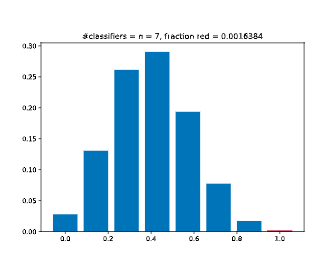
\includegraphics[width=\textwidth,height=\textheight,keepaspectratio]{lecture8_all_wrong}
    \end{center}

    \begin{remark}
        Of course, if we employ an ensemble classification, then we will use the majority
        label over the ensemble's models, so the relevant question is: what is the
        probabiliy that more than half the classifiers mispredict? Again, however,
        we see from the diagram below that this phenomenon is less and less likely
        the greater $n$ is.
    \end{remark}

    \begin{center}
        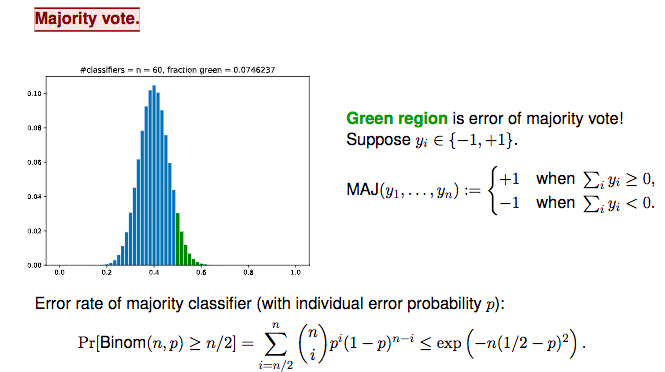
\includegraphics[width=\textwidth,height=\textheight,keepaspectratio]{lecture8_half_wrong}
    \end{center}

    \subsection{Bagging and Random Forests}


    \begin{remark}
        We explored a deterministic rule for constructing a tree. Therefore, the idea
        of constructing multiple trees as classifiers is nonsensical. There is a remedy
        called bagging, however. Critical to bagging is the idea that we can construct
        random datasets over which to make our model using sampling with replacement:
    \end{remark}

    \begin{center}
        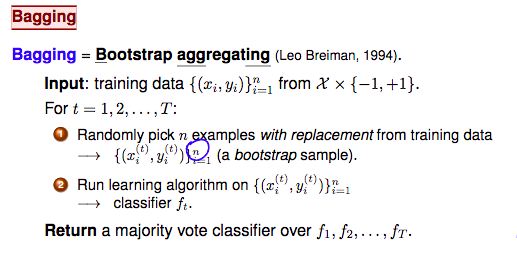
\includegraphics[width=\textwidth,height=\textheight,keepaspectratio]{lecture8_bagging}
    \end{center}

    \begin{remark}
        A random forest is a particular adapation of bagging to decision trees (note that
        bagging, above, was not particular to decision trees) in which we construct
        trees not only over a random sample of data but over a random subset of $\sqrt{d}$
        features:
    \end{remark}

    \begin{center}
        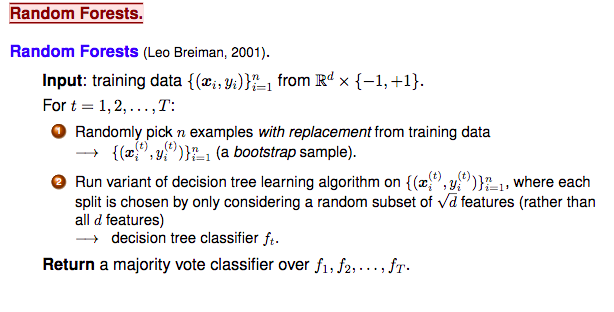
\includegraphics[width=\textwidth,height=\textheight,keepaspectratio]{lecture8_random_forest}
    \end{center}

    \subsection{Boosting}

    \begin{definition}
        Assume that we have a weak learning oracle (WLO) that, given a reweighted
        dataset (a dataset $\mc{D}$ with a probability assigned to each point),
        gives us a weak classifier with error $1/2 - \gamma$ for some $\gamma > 0$. Then
        do the following:
    \end{definition}

    \begin{center}
        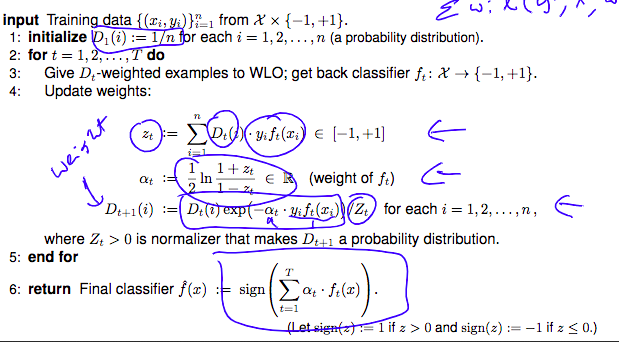
\includegraphics[width=\textwidth,height=\textheight,keepaspectratio]{lecture8_boost}
    \end{center}

    \begin{remark}
        We give some intuition for why AdaBoost is favorable:

        We can motivate this as if it were a problem:

        \begin{problem}{1}
            Suppose that $(X,Y) \sim D_t$ (this means that $(X,Y)$ obey the distribution
            $D_t$). Suppose that we have a weak classifier $f_t$ such that
            \[
                \bb{P}(f_{t}(X) = Y) = \frac{1}{2} + \gamma_t
            \]

            Then show that

            \[
                \sum_{i=1}^{n}D_{t}(i)\left(y_{i}f_{t}(x_{i}) \right) \geq 2\gamma_t
            \]

            Hint: the claim
            \[
                \bb{P}(f_{t}(X) = Y) = \frac{1}{2} + \gamma_t
            \]

            is ``approximately'' equivalent to the claim that

            \[
                \sum_{i=1}^{n}\delta(y^{i} = f(x_i))D_t(i) \geq \frac{1}{2} + \gamma_t
            \]
        \end{problem}

        \begin{proof}
            
            Observe that

            \begin{align*}
                \sum_{i=1}^{n}\delta(y^{i} = f(x_i))D_t(i) \geq \frac{1}{2} + \gamma_t \\
                \implies \sum_{i=1}^{n}\delta(y^{i} \not = f(x_i))D_t(i) \leq \frac{1}{2} - \gamma_t \\
                \implies \sum_{i \st y_i f(x_i) = -1}^{}(-1)D_t(i) \geq \gamma_t - \frac{1}{2} \\
                \intertext{Similarly:} \\
                \sum_{i \st y_i f(x_i) = 1}^{}(1)D_t(i) \geq \gamma_t + \frac{1}{2} \\
                \intertext{Combining the foregoing too, we get} \\
                \sum_{i \st y_i f(x_i) = 1}^{}(1)D_t(i) + \sum_{i \st y_i f(x_i) = -1}^{}(-1)D_t(i) = \sum_{i=1}^{n}D_t(i)(y_{i}f(x_{i})) \geq \gamma_t + \frac{1}{2} + \gamma_t - \frac{1}{2} = 2 \gamma_t \\
            \end{align*}
        \end{proof}<++>


        \breathe
    \begin{center}
        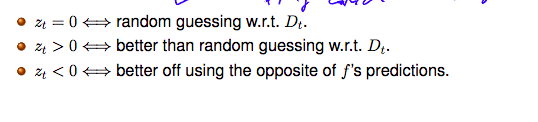
\includegraphics[width=\textwidth,height=\textheight,keepaspectratio]{lecture8_z}
    \end{center}

        Recall that 

        \[
            z_t = \sum_{i=1}^{n}D_t(i)(f_t(x_i)y_{i})
        \]

        We are weighing correctness $(+1)$ and incorrectness $(-1)$ by the probabilities
        that either correctness or incorrectness take place with.

        So that a positive $z_t$ signals prediction better than random guessing in the 
        world defined by $D_t$, $z_t = 0$ signals random guessing and negative $z_t$
        signals prediction worse than random guessing.

        Once we calculate $z_t$, if $z_t$ is positive (meaning, again, that we are doing a better
        job than normal), we effectively set $\alpha_t$ to be positive and negative
        otherwise (ie if $z_t$ is negative). $\alpha_t$ will then divert training attention
        accordingly in the next round of AdaBoost.

    \begin{center}
        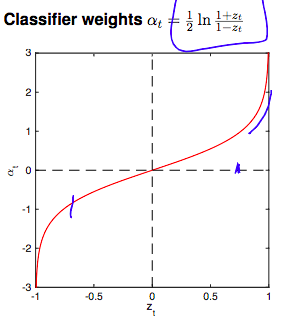
\includegraphics[width=\textwidth,height=\textheight,keepaspectratio]{lecture8_alpha}
    \end{center}

    Now recall that $D_{t+1}(i) = D_{t}(i) \exp{(-\alpha_i \cdot y_i f_t(x_i))}/Z_{t}$,
    sot hat we give a higher weight to data points that were misclassified than to those
    that were well classified.
    \end{remark}


    \begin{remark}
    \begin{center}
        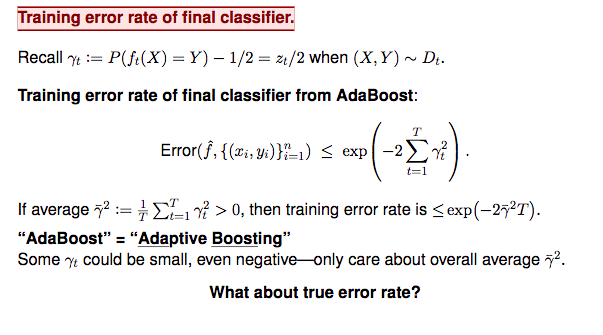
\includegraphics[width=\textwidth,height=\textheight,keepaspectratio]{lecture8_ada_holistic}
    \end{center}

    The first line is really a manipulation of the previously proven fact that
    if $z_t = \sum_{i=1}^{n}D_{t}(i)[y_{i}f_{t}(x_{i})]$ and if 
    \[
        \frac{1}{2} + \gamma_t = \bb{P}(f_t(X) = Y) \approx \sum_{i=1}^{n}D_{t}(i) \delta[y_{i} = f(x_{i})]
    \]

    then we can say $z_t = 2 \gamma_t$. Clearly then, it is true, as the line asserts, that

    \[
    \bb{P}(f_{t}(X) = Y) = \gamma_t + \frac{1}{2} = \frac{2\gamma_t + 1}{2} = \frac{z_{t} + 1}{2}    \]


    The other lines are black boxes that we must take for granted. Importantly, the error
    of the classifier that adaboost would give us at iteration $T$ is bounded exponentially
    by the averages of $\gamma_t^2$ for $t \in \{1 \dots T\}$. This measn that even if
    some $\gamma_t$ are negative, that is okay: we care that the average be positive.

    \begin{center}
        
\includegraphics[width=\textwidth,height=\textheight,keepaspectratio]{lecture8_ada_final}
    \end{center}

    When we finish with Ada Boost, we get this final predictor above. UNRESOLVED: why do
    larger SVM margins imply better resistance to overfitting.
    \end{remark}





\end{document}










